%Every LaTeX file needs a documentclass declaration.
%Possibilities are article, book, letter.  Font size is also declared.

\documentclass[10pt]{article}

%special packages used for symbols, formatting, etc.

\usepackage{amsmath} % contains the align* environment, which is great for manipulating formulas
\usepackage{amssymb} % contains common symbols
\usepackage{amsthm} % has the proof environment
\usepackage[margin=1in]{geometry} % specifies page properties, such as the margin
%\usepackage{siunitx} % useful for typesetting units
\usepackage{tikz} % useful for graphics

% Define a lemma environment
% Set the style of the new theorem environments so that the text isn't in italics
\theoremstyle{definition}
% Define lemma environment, the first argument is the name in LaTeX, the second argument is what is typeset
\newtheorem{lemma}{Lemma}

% User-defined commands

\newcommand{\newprob}{\medskip \hrule \medskip}
\newcommand{\fanc}[1]{\mathbb{#1}}
\newcommand{\rn}[1]{\fanc{R}^{#1}}
\def\qed{\hspace*{\fill}\rule{1.854mm}{3mm}}  % the fancy box at the end of a proof

%%%%%%%%%%%%%%%%%%%%%%%%%%%%%%%%%%%%%%%%%%%%%%

%beginning of document, every \begin{} also requires an \end{} command.

%\renewcommand{\baselinestretch}{2}

\begin{document}

\pagestyle{empty}  %suppress page numbers, etc.

\begin{center}  %center command, also see flushright, flushleft

{\bf MATH 423-01  Advanced Calculus I

Homework \#7

Assigned: November 3, 2022

Due: November 10, 2022}

\end{center}

\medskip

\hrule   %horizontal line

\bigskip

% list environment: description, itemize, and enumerate

\begin{enumerate}

%%%%%%%%%%%%%%%%%%%%%%

\item  Use the definition of continuity to prove the following statements.

	\begin{enumerate}
	
	\item  ~[Papiernik, J.] $$\lim_{x \to 2} (2x+4) = 8$$
	
	\item  ~[Powers, S.] $$\lim_{x \to 1} (x^3-1) = 0$$
	
	\item  ~[Schipke, K.] $$\lim_{x \to 2} x^3 = 8$$
	
	\item  ~[Schmidt, S.] $$\lim_{x \to \pi} \lfloor x \rfloor = 3,$$ where $\lfloor x \rfloor$ denotes the greatest integer less than or equal to $x$, otherwise known as the ``floor'' function.
	
	\end{enumerate}
	
%%%%%%%%%%%%

\item  ~[Smith, G.] Use the Criterion for Discontinuity from the notes to show that each of the following limits do not exist.

	\begin{enumerate}
	
	\item  $$\lim_{x \to 0} \frac{|x|}{x}$$
	
	\item  $$\lim_{x \to 1} g(x),$$ where $g(x)$ is Dirichlet's function.
	
	\end{enumerate}
	
%%%%%%%%%%%%
	
\item  ~[Wright, A.] Review the definition of Thomae's function, $t(x)$.

	\begin{enumerate}
	
	\item  Construct three different sequences, $(x_n)$, $(y_n)$, and $(z_n)$, each of which converges to $1$ without using the number $1$ as a term in the sequence.
	
	\item  Compute $\lim{(t(x_n))}$, $\lim{(t(y_n))}$, and $\lim{(t(z_n))}$.
	
	\item  Make an educated conjecture for $$\lim_{x \to 1} t(x).$$ %and use the topological definition of continuity to verify the claim.	
	
	\end{enumerate}
	
%%%%%%%%%%%%%

\item  ~[Aitchison, A.]

	\begin{enumerate}
	
	\item  The statement $$\lim_{x \to 0} \frac{1}{x^2} = \infty$$ makes intuitive sense.  Construct a rigorous definition for a limit statement of the form $$\lim_{x \to c} f(x) = \infty$$ using ideas like $N$, $\delta$, and $\varepsilon$, and use it to prove the limit statement concerning $1/x^2$.
	
	\item  Construct a definition for the statement $$\lim_{x \to \infty} f(x) = L.$$ Show that $$\lim_{x \to \infty} \frac{1}{x} = 0.$$
	
	\item  What would the definition of $$\lim_{x \to \infty} f(x) = \infty$$ look like?  Give an example of such a limit.
	
	\end{enumerate}
	
%%%%%%%%%%%%%%

\item  ~[Hale, A.] (Squeeze Theorem)  Let $f$, $g$, and $h$ satisfy $f(x) \leq g(x) \leq h(x)$, for all $x$ in a common domain, $A$.  If $$\lim_{x \to c} f(x) = \lim_{x \to c} h(x) = L$$ at some limit point of $A$, prove that $$\lim_{x \to c} g(x) = L.$$

Hint: don't start from scratch.  We already have a Squeeze Theorem for sequences (Homework \#4).  Use it.

%%%%%%%%
	
\item  ~[Harter, J.] Let $f: A \to \mathbb{R}$ and $g: B \to \mathbb{R}$, such that $f(A) \subseteq B$.  If $f$ is continuous at $c \in A$ and $g$ is continuous at $f(c) \in B$, prove that $(g \circ f)(x)$ is continuous at $c$.  Use a $\delta$-$\varepsilon$ proof.
	
%%%%%%%%%%
	
\item  ~[Everyone, James, J.] (\textbf{Topological Characterization of Continuity})  Let $g: X \to Y$.  If $A \subseteq Y$ is in the co-domain of $g$, define $$g^{-1}(A) = \{x \in X: g(x) \in Y \},$$ which we previously defined as the pre-image of $A$.  Note that $g^{-1}(A) \subseteq X$. Prove that $g$ is continuous if and only if $g^{-1}(\Omega)$ is an open set in $X$ whenever $\Omega$ is an open set in $Y$.

Hint: this is a hard problem because there are many sets and neighborhoods in the same problem, some in the domain and some in the range.  Rely on definitions, and make sure that you apply them in the proper order.  For instance, if you need to prove that a set is open, don't start with the definition of continuity.
	
%%%%%%%%%%%%

\item  In class we used the Heine-Borel Theorem to prove the Extreme Value Theorem (EVT).  This is another statement that can be used to prove all of the other statements we have proven so far.  This updates Figure \ref{fig:theorems}.

	\begin{figure}[h]
	\begin{center}
	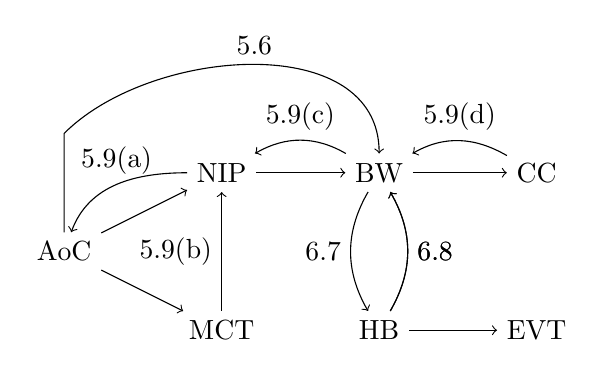
\begin{tikzpicture}
	
	% Draw nodes
	\node (AoC) at (0,0) {AoC};
	\node (MCT) at (2,-1) {MCT};
	\node (NIP) at (2,1) {NIP};
	\node (BW) at (4,1) {BW};
	\node (CC) at (6,1) {CC};
	\node (HB) at (4,-1) {HB};
	\node (EVT) at (6,-1) {EVT};
	
	% Draw arcs, what we have proved in class or the homework
	\draw[->] (AoC) to (MCT);
	\draw[->] (AoC) to (NIP);
	\draw[->] (NIP) to (BW);
	\draw[->,in=90] (AoC) |- (0,1.5) to node[midway,above] {5.6} (BW);
	\draw[->] (BW) to (CC);
	\draw[->,out=180,in=70] (NIP) to node[midway,above] {5.9(a)} (AoC);
	\draw[->] (MCT) to node[midway,left] {5.9(b)} (NIP);
	\draw[->,out=150,in=30] (BW) to node[midway,above] {5.9(c)} (NIP);
	\draw[->,out=150,in=30] (CC) to node[midway,above] {5.9(d)} (BW);
	\draw[->,out=-120,in=120] (BW) to node[midway,left] {6.7} (HB);
	\draw[->,out=60,in=-60] (HB) to node[midway,right] {6.8}  (BW);
	
	% Draw arcs, what we will prove here
	\draw[->] (HB) to (EVT);
	\draw[->,out=60,in=-60] (HB) to node[midway,right] {6.8}  (BW);
	
	\end{tikzpicture}
	\caption{A directed graph showing the logical implications of the various statements.}\label{fig:theorems}
	\end{center}
	\end{figure}
	
	%%%%%%%%%
	
I have not had time to figure out how to show that the Extreme Value Theorem can be used to prove any of the other theorems.  Part of my problem is that the Extreme Value Theorem involves the range of a function, while the other statements involve sets or sequences in sets.  This problem offers extra credit to anyone who can show that the Extreme Value Theorem can be used to prove any of the other six statements in Figure \ref{fig:theorems}.  You can look anywhere you want for inspiration, but you have to document your sources.  This extra credit problem will remain in existence until either the end of the semester or until I can find a proof.  Be careful, though.  People have showed that these statements are logically equivalent using contrapositive and counterexamples.  I am looking for a proof, not counterexamples.
	
%%%%%%%%%%%%%

\end{enumerate}

\end{document}
